\documentclass[10pt, a4paper, english]{../Template/NTNUoving}
\usepackage[utf8]{inputenc}
\usepackage[T1]{fontenc}
\usepackage{float}
\usepackage{enumitem}
\usepackage{csquotes}
\usepackage{algorithm}
\usepackage{algorithmic}
\usepackage{listings}
\usepackage{listings}
\usepackage{color}
\usepackage{biblatex}
\usepackage{hyperref}
\ovingnr{1}    % Nummer på innlevering
\semester{Spring 2021}
\fag{Methods in Artificial Intelligence \\ TDT4171}
\institutt{Department for Computer Science}

\begin{document}

% Problem 1
\begin{oppgave}

    % a
    \begin{punkt}
        \begin{align*}
            P(Siblings \leq 2)
            &= P(Siblings = 0) + P(Siblings = 1) + P(Siblings = 2) \\
            &= 0.15 + 0.49 + 0.27 \\
            &= 0.91
        \end{align*}
    \end{punkt}

    % b
    \begin{punkt}
        \begin{align*}
            P(Siblings > 2 | Siblings \geq 1)
            &= \frac{P(Siblings > 2 \wedge Siblings \geq 1)}{P(Siblings \geq 1)} \\
            &= \frac{P(Siblings > 2)}{P(Siblings \geq 1)} \\
            &= \frac{1-P(Siblings \leq 2)}{1-P(Siblings = 0)} \\
            &= \frac{0.09}{0.85} = \frac{9}{85} \approx 0.1059
        \end{align*}
    \end{punkt}

    % c
    \begin{punkt}
        Let $S_1$, $S_2$ and $S_3$ denote the siblings for each of the friends.

        There are 3 permutations for who can have 3 siblings and the other 0 siblings,
        only 1 permutation where each have 1 sibling and $3\cdot2=6$ permutations for who can have 2 siblings, 1 sibling and 0 sibling
        (we first have 3 choices for the friend with 2 siblings, then 2 choices for the one with 1 sibling).
        This gives us:

        \begin{align*}
            P(S_1 + S_2 + S_3 = 3)
            &= 3P(S_1 = 3)P(S_2 = 0)P(S_3 = 0) \\
            &+ P(S_1 = 1)P(S_2 = 1)P(S_3 = 1) \\
            &+ 6P(S_1 = 2)P(S_2 = 1)P(S_3 = 0) \\
            &= 3\cdot0.06\cdot0.15^2 + 0.49^3 + 6\cdot0.27\cdot0.49\cdot0.15\\
            &= 0.240769
        \end{align*}
    \end{punkt}

    % d
    \begin{punkt}
        Let $S_E$ and $S_J$ denote siblings for Emma and Jacob respectfully. We have:
        \begin{align*}
            P(S_E = 0 | S_E + S_J = 3)
            &= \frac{P(S_E = 0 \wedge S_E + S_J = 3)}{P(S_E + S_J = 3)} \\
            P(S_E = 0 \wedge S_E + S_J = 3) &= P(S_E = 0)P(S_J = 3) \\
            P(S_E + S_J = 3) &= 2 P(S_E = 0)P(S_J = 3) + 2 P(S_E = 1)P(S_J = 2) \\
            \implies P(S_E = 0 | S_E + S_J = 3) &= \frac{P(S_E = 0)P(S_J = 3)}{2 P(S_E = 0)P(S_J = 3) + 2 P(S_E = 1)P(S_J = 2)} \\
            &= \frac{0.15\cdot0.06}{2\cdot0.15\cdot0.06 + 2\cdot0.49\cdot0.27} \\
            &= \frac{5}{157} \approx 0.031847
        \end{align*}
    \end{punkt}
\end{oppgave}

% Problem 2
\begin{oppgave}
    %a
    \begin{punkt}
        Every node can be represented by $2^k$ numbers where $k$ is the number of parent nodes when each variable has a Boolean state.
        This gives us the following:
        \begin{center}
            \begin{tabular}{ |c|c| }
             \hline
             Variable & Numbers needed \\
             \hline
             A  & 1 \\
             \hline
             B &  2 \\
             \hline
             C &  2 \\
             \hline
             D &  2 \\
             \hline
             E &  4 \\
             \hline
             F &  4 \\
             \hline
             G &  2 \\
             \hline
             H &  1 \\
             \hline
             Sum &  18 \\
             \hline
            \end{tabular}
            \end{center}
            As we can see the sum is 18 numbers needed and the statement is thus \textbf{true}.
    \end{punkt}

    For solving the next exercises I will use d-separation as described in \href{http://web.mit.edu/jmn/www/6.034/d-separation.pdf}{this document from MIT}.
    Since d-separation is a sufficient condition for conditional independence, we can use this to determine if the statements are false or true with the given knowledge about the Bayesian network.

    % b
    \begin{punkt}
        \textbf{True}, we can see that $G$ and $A$ are d-separated in \ref{fig:2b}.
        \begin{figure}[H]
            \centering
            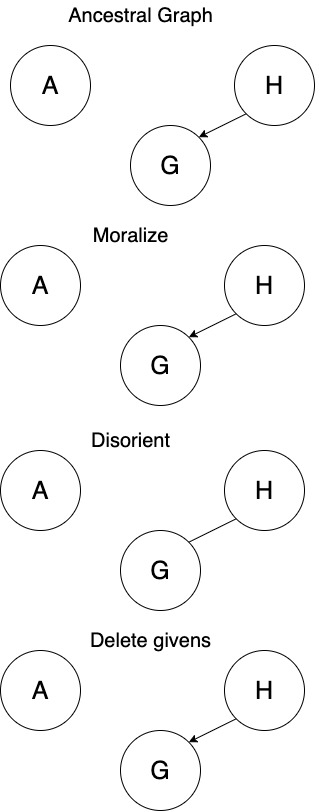
\includegraphics[width=0.5\textwidth]{Task2b.png}
            \caption{Using d-separation to determine independence for $G \perp A$.}
            \label{fig:2b}
            \end{figure}
    \end{punkt}

    % c
    \begin{punkt}
        \textbf{True}, we can see that $E$ and $H$ are d-separated in \ref{fig:2c}.
        \begin{figure}[H]
            \centering
            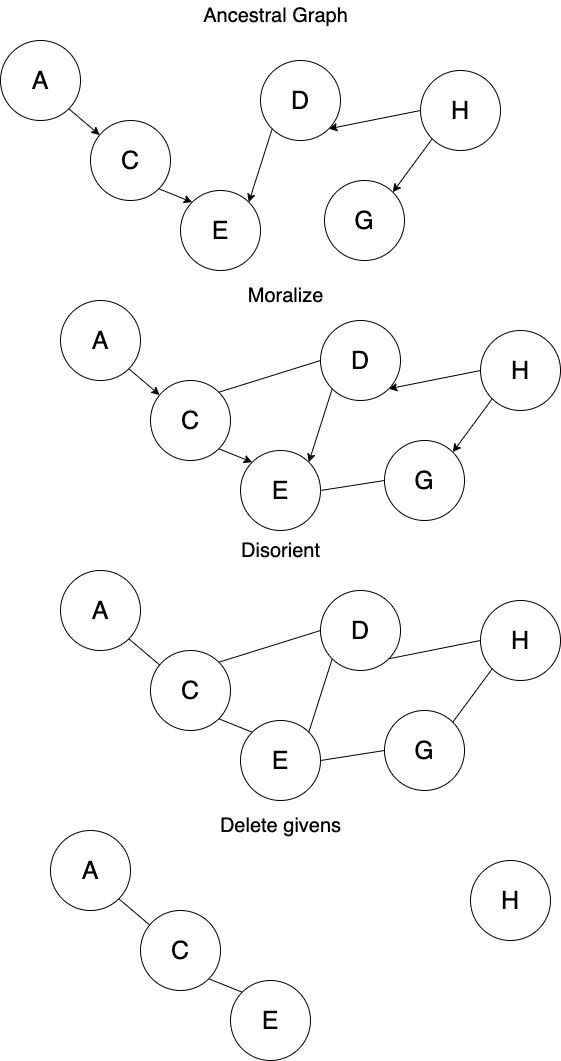
\includegraphics[width=0.5\textwidth]{Task2c.png}
            \caption{Using d-separation to determine independence for $E \perp H | \{D, G\}$.}
            \label{fig:2c}
            \end{figure}
    \end{punkt}

    % d
    \begin{punkt}
        \textbf{False}, we can see that $E$ and $H$ are \textbf{not} d-separated in \ref{fig:2d}. This means that we cannot \textbf{guarantee} independence. However, the specific
        probabilities involved could make them indepedent, but since we are given none probability tables we don't have enough information to determine this.
        \begin{figure}[H]
            \centering
            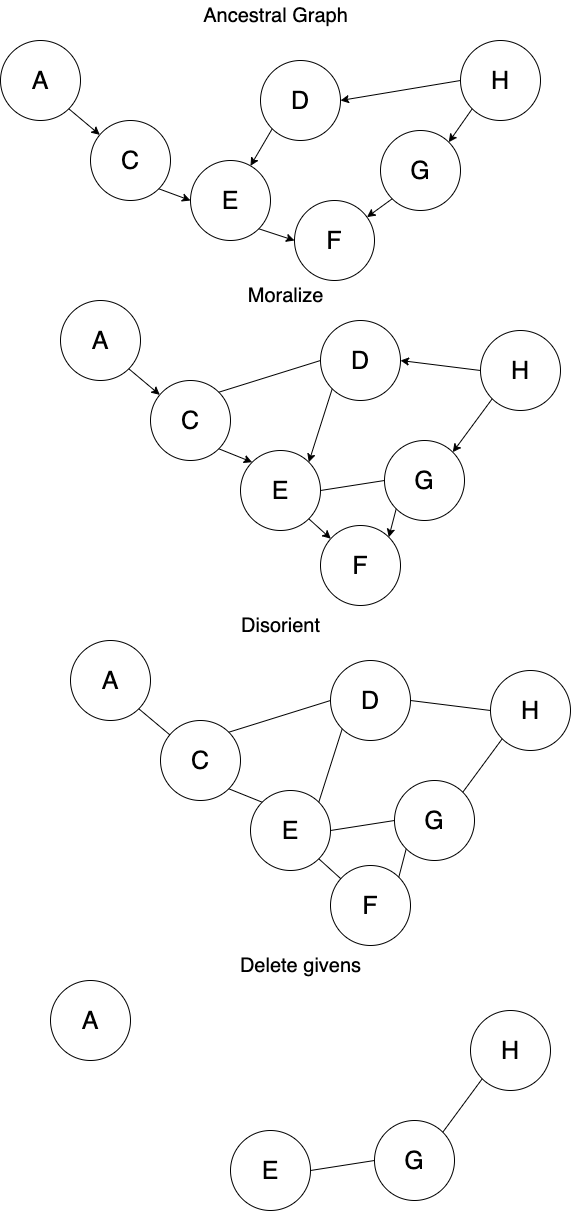
\includegraphics[width=0.5\textwidth]{Task2d.png}
            \caption{Using d-separation to determine independence for $E \perp H | \{C, D, F\}$.}
            \label{fig:2d}
            \end{figure}
    \end{punkt}
\end{oppgave}

% Problem 3
\begin{oppgave}

    % a
    \begin{punkt}
        \begin{align*}
            P(b) &=
            P(b|a)P(a)+P(b|\neg a)P(\neg a) \\
            &= 0.44 \\
            \implies P(\neg b) &= 1-P(b) = 0.56
        \end{align*}
    \end{punkt}

     % b
     \begin{punkt}
        \begin{align*}
            P(d) &=
            P(d|b)P(b)+P(d|\neg b)P(\neg b) \\
            &= 0.712 \\
        \end{align*}
     \end{punkt}

      % c
    \begin{punkt}
        \begin{align*}
            P(B | \neg d)
            &= \alpha \langle P(\neg d|b)P(b), P(\neg d | \neg b)P(\neg b) \rangle \\
            &= \alpha \langle \frac{22}{125}, \frac{14}{125} \rangle = \langle \frac{11}{18}, \frac{7}{18}\rangle \\
            \implies P(c|\neg d) &= P(c|b)P(b|\neg d) +  P(c|\neg b)P(\neg b|\neg d) \\
            &= \frac{11}{180} + \frac{7}{60} = \frac{8}{45} \approx 0.178
        \end{align*}
        $\alpha$ is the normalizing factor.
    \end{punkt}

     % d
     \begin{punkt}
        \begin{align*}
            P(A | \neg c, d)
            &= \alpha \langle P(a)\sum_b P(\neg b|a)P(\neg c |b) P(d|b), P(\neg a)\sum_b P(\neg b|\neg a)P(\neg c |b) P(d|b) \rangle \\
            &= \alpha \langle \frac{11}{25}, \frac{139}{1250} \rangle = \langle \frac{550}{689}, \frac{139}{689} \rangle \approx \langle 0.7983, 0.2017 \rangle
        \end{align*}
        $\alpha$ is the normalizing factor.
     \end{punkt}
\end{oppgave}
\clearpage
% Problem 4
\begin{oppgave}
    % c
    \setcounter{Punkt}{2}
    \begin{punkt}
        The Monty-Hall problem can be described by a bayesian network where $OpenedByHost$ is conditional based on $Prize$ and $ChosenByGuest$:

        \begin{figure}[h]
            \centering
            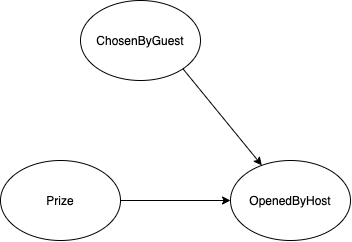
\includegraphics[width=0.5\textwidth]{BN.png}
            \caption{Bayesian network for the Monty Hall-problem.}

            \end{figure}

        The following logic was used when constructing the probability tables:

        \begin{itemize}
            \item The prize is chosen randomly between the 3 doors giving a probability of $1/3$ to each.
            \item The guest is choosing randomly between the 3 doors also giving a probability of $1/3$ to each.
            \item The door opened by the host is determined based on the choices of prize and guest, both of which the host knows. The host will never chose
            the door chosen by prize and guest so the probability of these doors are always 0. Otherwise we have two cases:
            \begin{enumerate}
                \item If the prize and guest has the same door, the host has two options, giving a probability of $1/2$ to both of them.
                \item If the prize and guest's door are not the same, the host only has one option left, giving a probability of $1$ to that door.
            \end{enumerate}
        \end{itemize}
        The conditional probability tables are then given by:
        \begin{table}[H]
            \centering
            \begin{tabular}{|c|c|}
                \hline
                & $P(Prize)$ \\ [0.5ex]
                \hline
                $Door1$ & 0.333 \\ [1.0ex]
                $Door2$ & 0.333 \\ [1.0ex]
                $Door3$ & 0.333 \\ [1.0ex]
                \hline
            \end{tabular}
            \caption{Probability distribution for $Prize$.}
        \end{table}

        \begin{table}[H]
            \centering
            \begin{tabular}{|c|c|}
                \hline
                & $P(ChosenByGuest)$ \\ [0.5ex]
                \hline
                $Door1$ & 0.333 \\ [1.0ex]
                $Door2$ & 0.333 \\ [1.0ex]
                $Door3$ & 0.333 \\ [1.0ex]
                \hline
            \end{tabular}
            \caption{Probability distribution for $ChosenByGuest$.}
        \end{table}

        \begin{table}[H]
            \centering
            \begin{tabular}{|c|c|c|c|c|c|c|c|c|c|}
                \hline
                $Prize$ & 0 & 1 & 2 & 0 & 1 & 2 & 0 & 1 & 2 \\ [1.0ex]
                $ChosenByGuest$ & 0 & 0 & 0 & 1 & 1 & 1 & 2& 2 & 2 \\ [1.0ex]
                \hline
                $Door1$ & 0 & 0 & 0 & 0 & 0.5 & 1 & 0 & 1  & 0.5 \\ [1.0ex]
                $Door2$ & 0.5 & 0 & 1 & 0 & 0 & 0 & 1 & 0 & 0.5 \\ [1.0ex]
                $Door3$ & 0.5 & 1 & 0 & 1 & 0.5 & 0 & 0 & 0 & 0 \\ [1.0ex]
                \hline
            \end{tabular}
            \caption{Probability distribution for $ChosenByGuest$.}
        \end{table}

        \begin{align*}
            P(Prize | ChosenByGuest = 1, OpenedByHost = 3) &= \langle 0.3333, 0.6667, 0.0000 \rangle
        \end{align*}
        Based on this it is of the interest of the guest to switch their choice.
    \end{punkt}
\end{oppgave}
\end{document}